\chapter{Les spécifications fonctionnelles et techniques}\label{ch:specifications-fonctionnelles-techniques}

J'ai travaillé sur le projet Pipeline documentaire sous la direction de ma tutrice au sein de l'équipe de développement de SuiviDeFlotte. Avant de commencer, étant donné la complexité du projet, nous avons tenu plusieurs réunions avec le propriétaire du produit. Celui-ci nous a expliqué en détail ses idées concernant le projet, et bien sûr, nous avons également partagé nos réflexions.

Dans le chapitre précédent, je crois que c'était évident que notre propriétaire de produit avait une vision précise de la manière dont l'application devait être construite et de son fonctionnement. Par conséquent, nous n'avons pas eu besoin de débuter par l'analyse d'un cahier des charges pour identifier les entités et les relations qu'il pourrait contenir. Cette étape avait déjà été accomplie.

Il a également été convenu que nous développerions ce projet en utilisant le framework Laravel et que nous le déploierions dans des conteneurs Docker. Nous avons constaté que le framework Laravel offrait tous les éléments nécessaires pour ce projet : commandes, gestion des événements, mise en file d'attente des tâches, ainsi que des fonctionnalités pour créer facilement une API, entre autres. De ce fait, ce choix nous est apparu comme judicieux, d'autant plus qu'il avait déjà été utilisé pour de nombreux autres projets au sein de la société, ce qui signifiait que les développeurs possédaient une solide expérience avec cet outil.

L'utilisation de conteneurs Docker pour le développement n'était pas encore une pratique courante au sein de l'entreprise. Cependant, une transition était prévue pour que tous les projets soient conteneurisés. Par conséquent, lors du lancement de nouveaux projets, leur conteneurisation était envisagée dès le début.

Au cours de ces réunions, de plus en plus de détails ont été précisés et nous étions prêts à entamer le projet. Néanmoins, il restait encore un travail de conception à accomplir pour définir en détail l'implémentation de ce projet dans ces cadres.

Le plan de mise en œuvre du projet dans le système de contrôleurs, de commandes et d'événements de Laravel est présenté dans le diagramme d'activités de la Figure~\ref{fig:import-activity-diagram}.

\begin{sidewaysfigure}
    \centering
    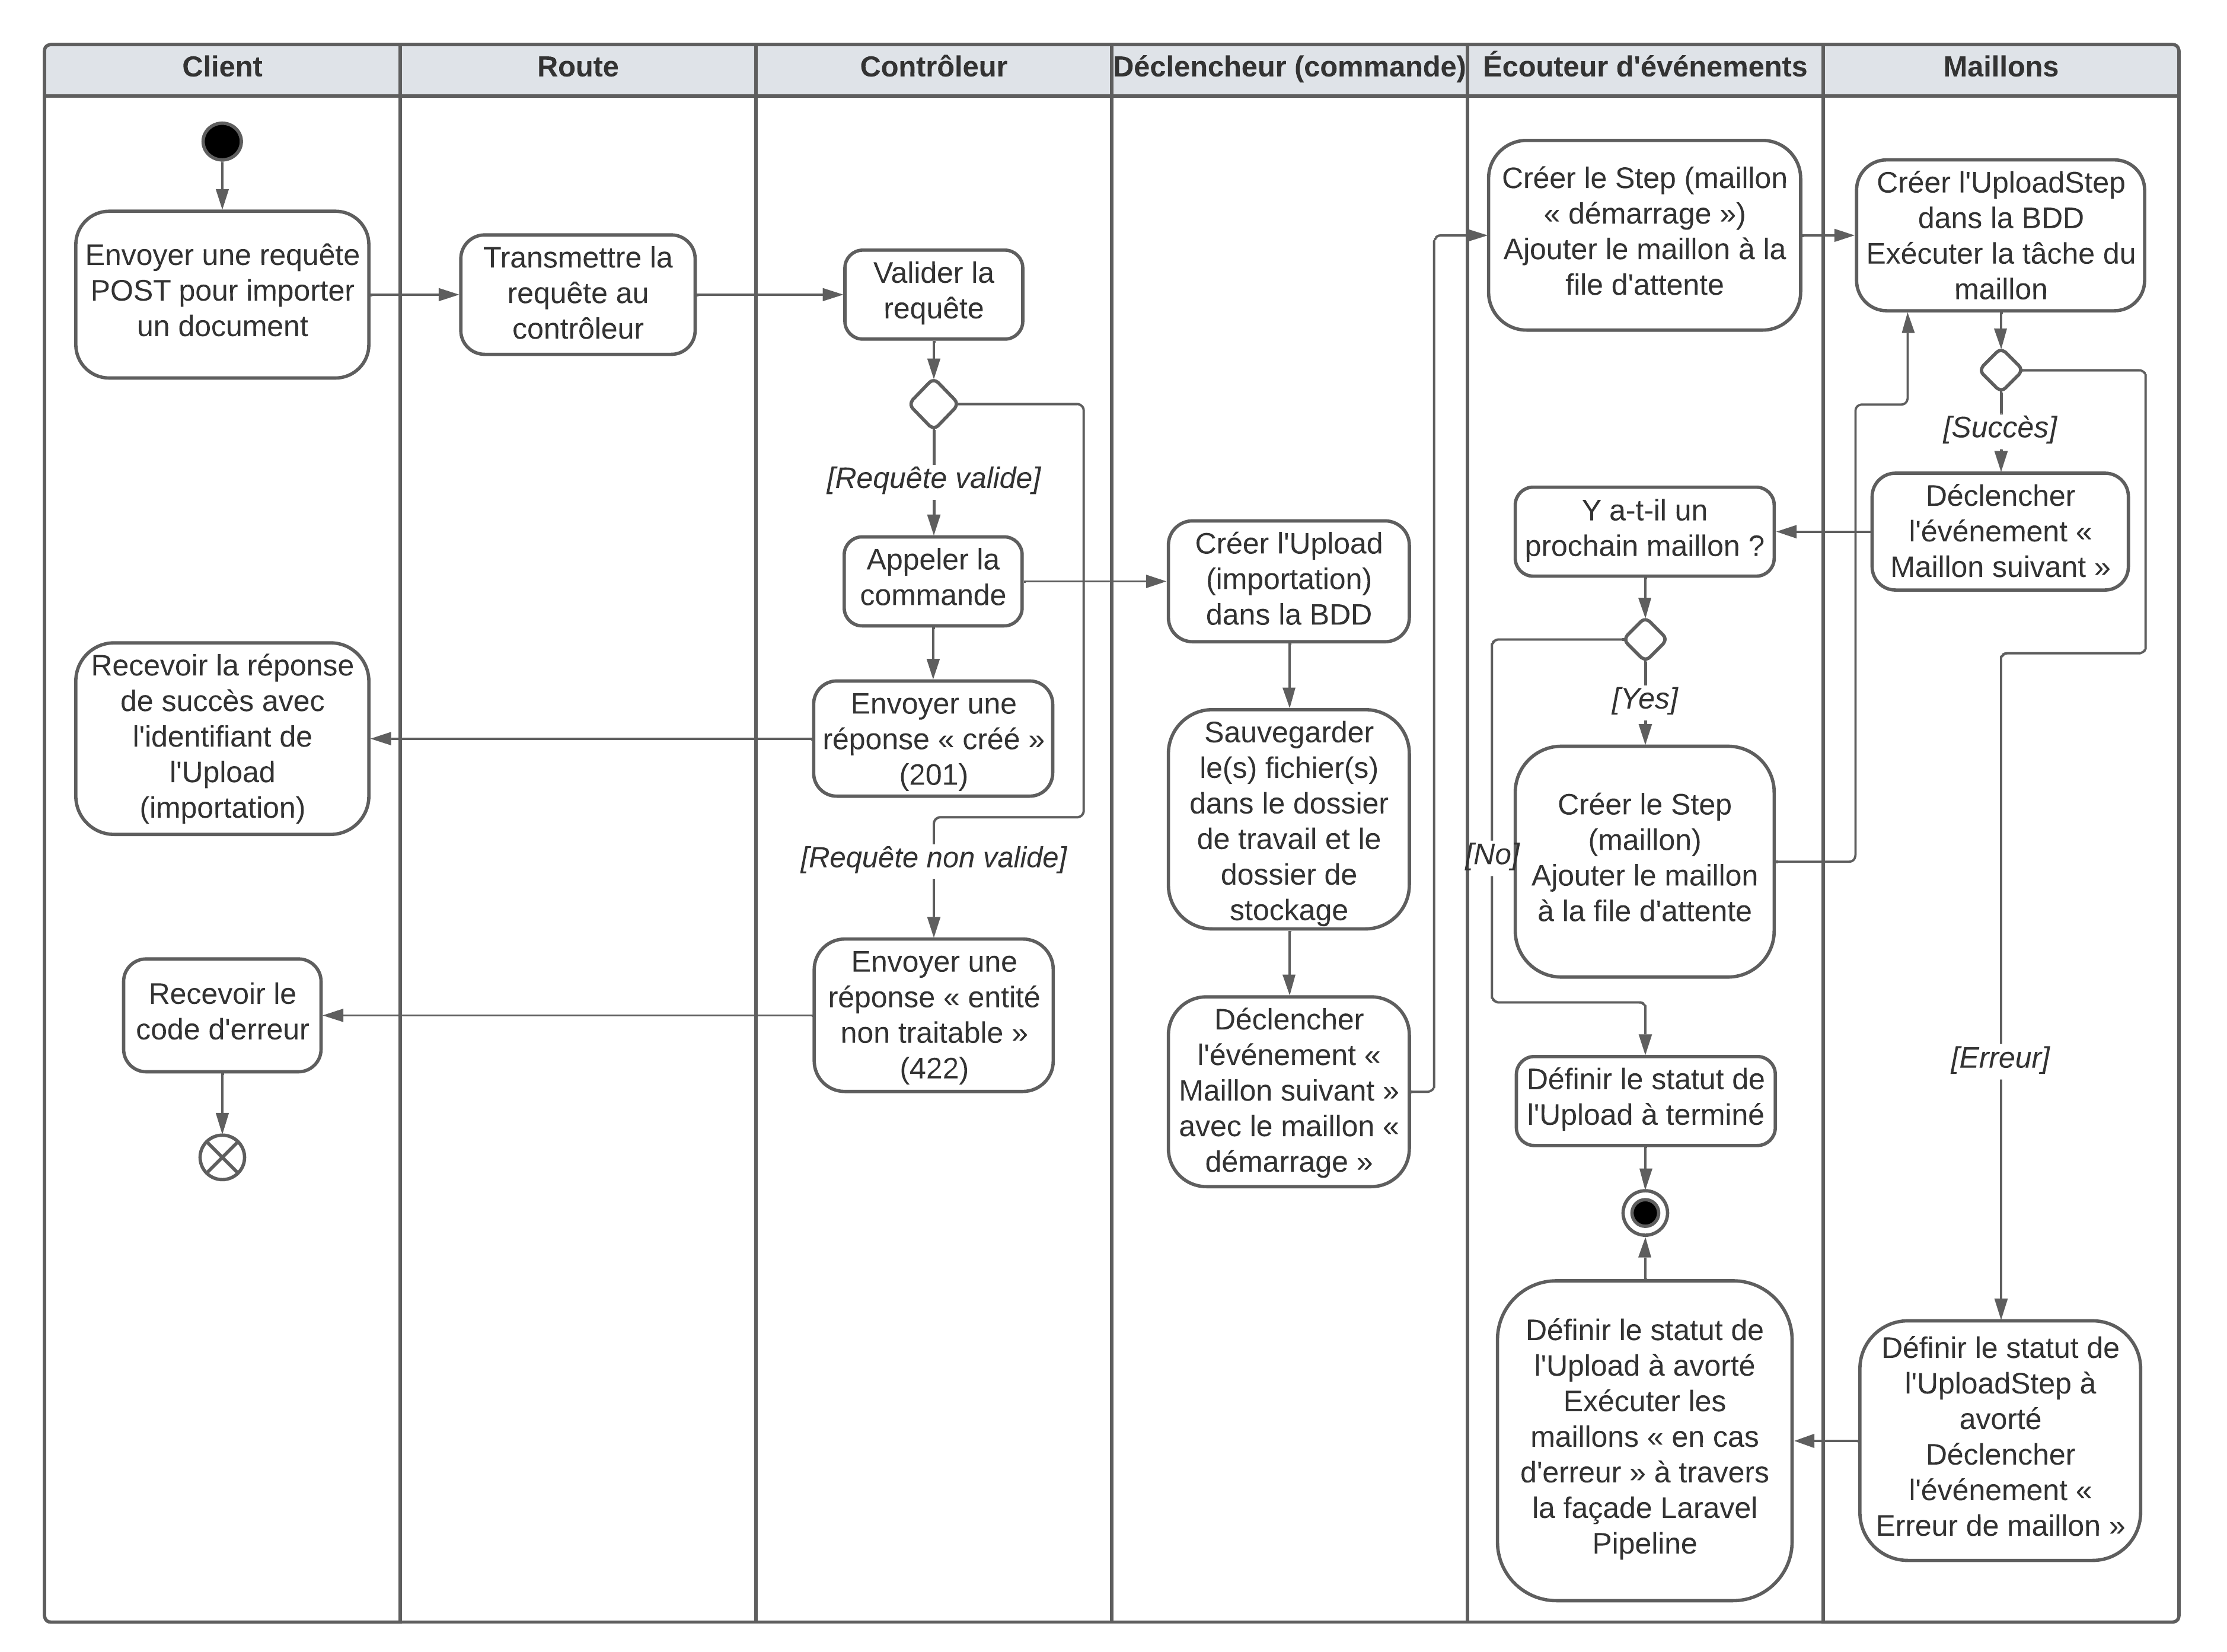
\includegraphics[width=\textwidth]{img/import-activity-diagram}
    \caption{Diagramme d'activité de l'envoi d'une requête POST pour importer un document.}
    \label{fig:import-activity-diagram}
\end{sidewaysfigure}

\begin{sidewaysfigure}
    \centering
    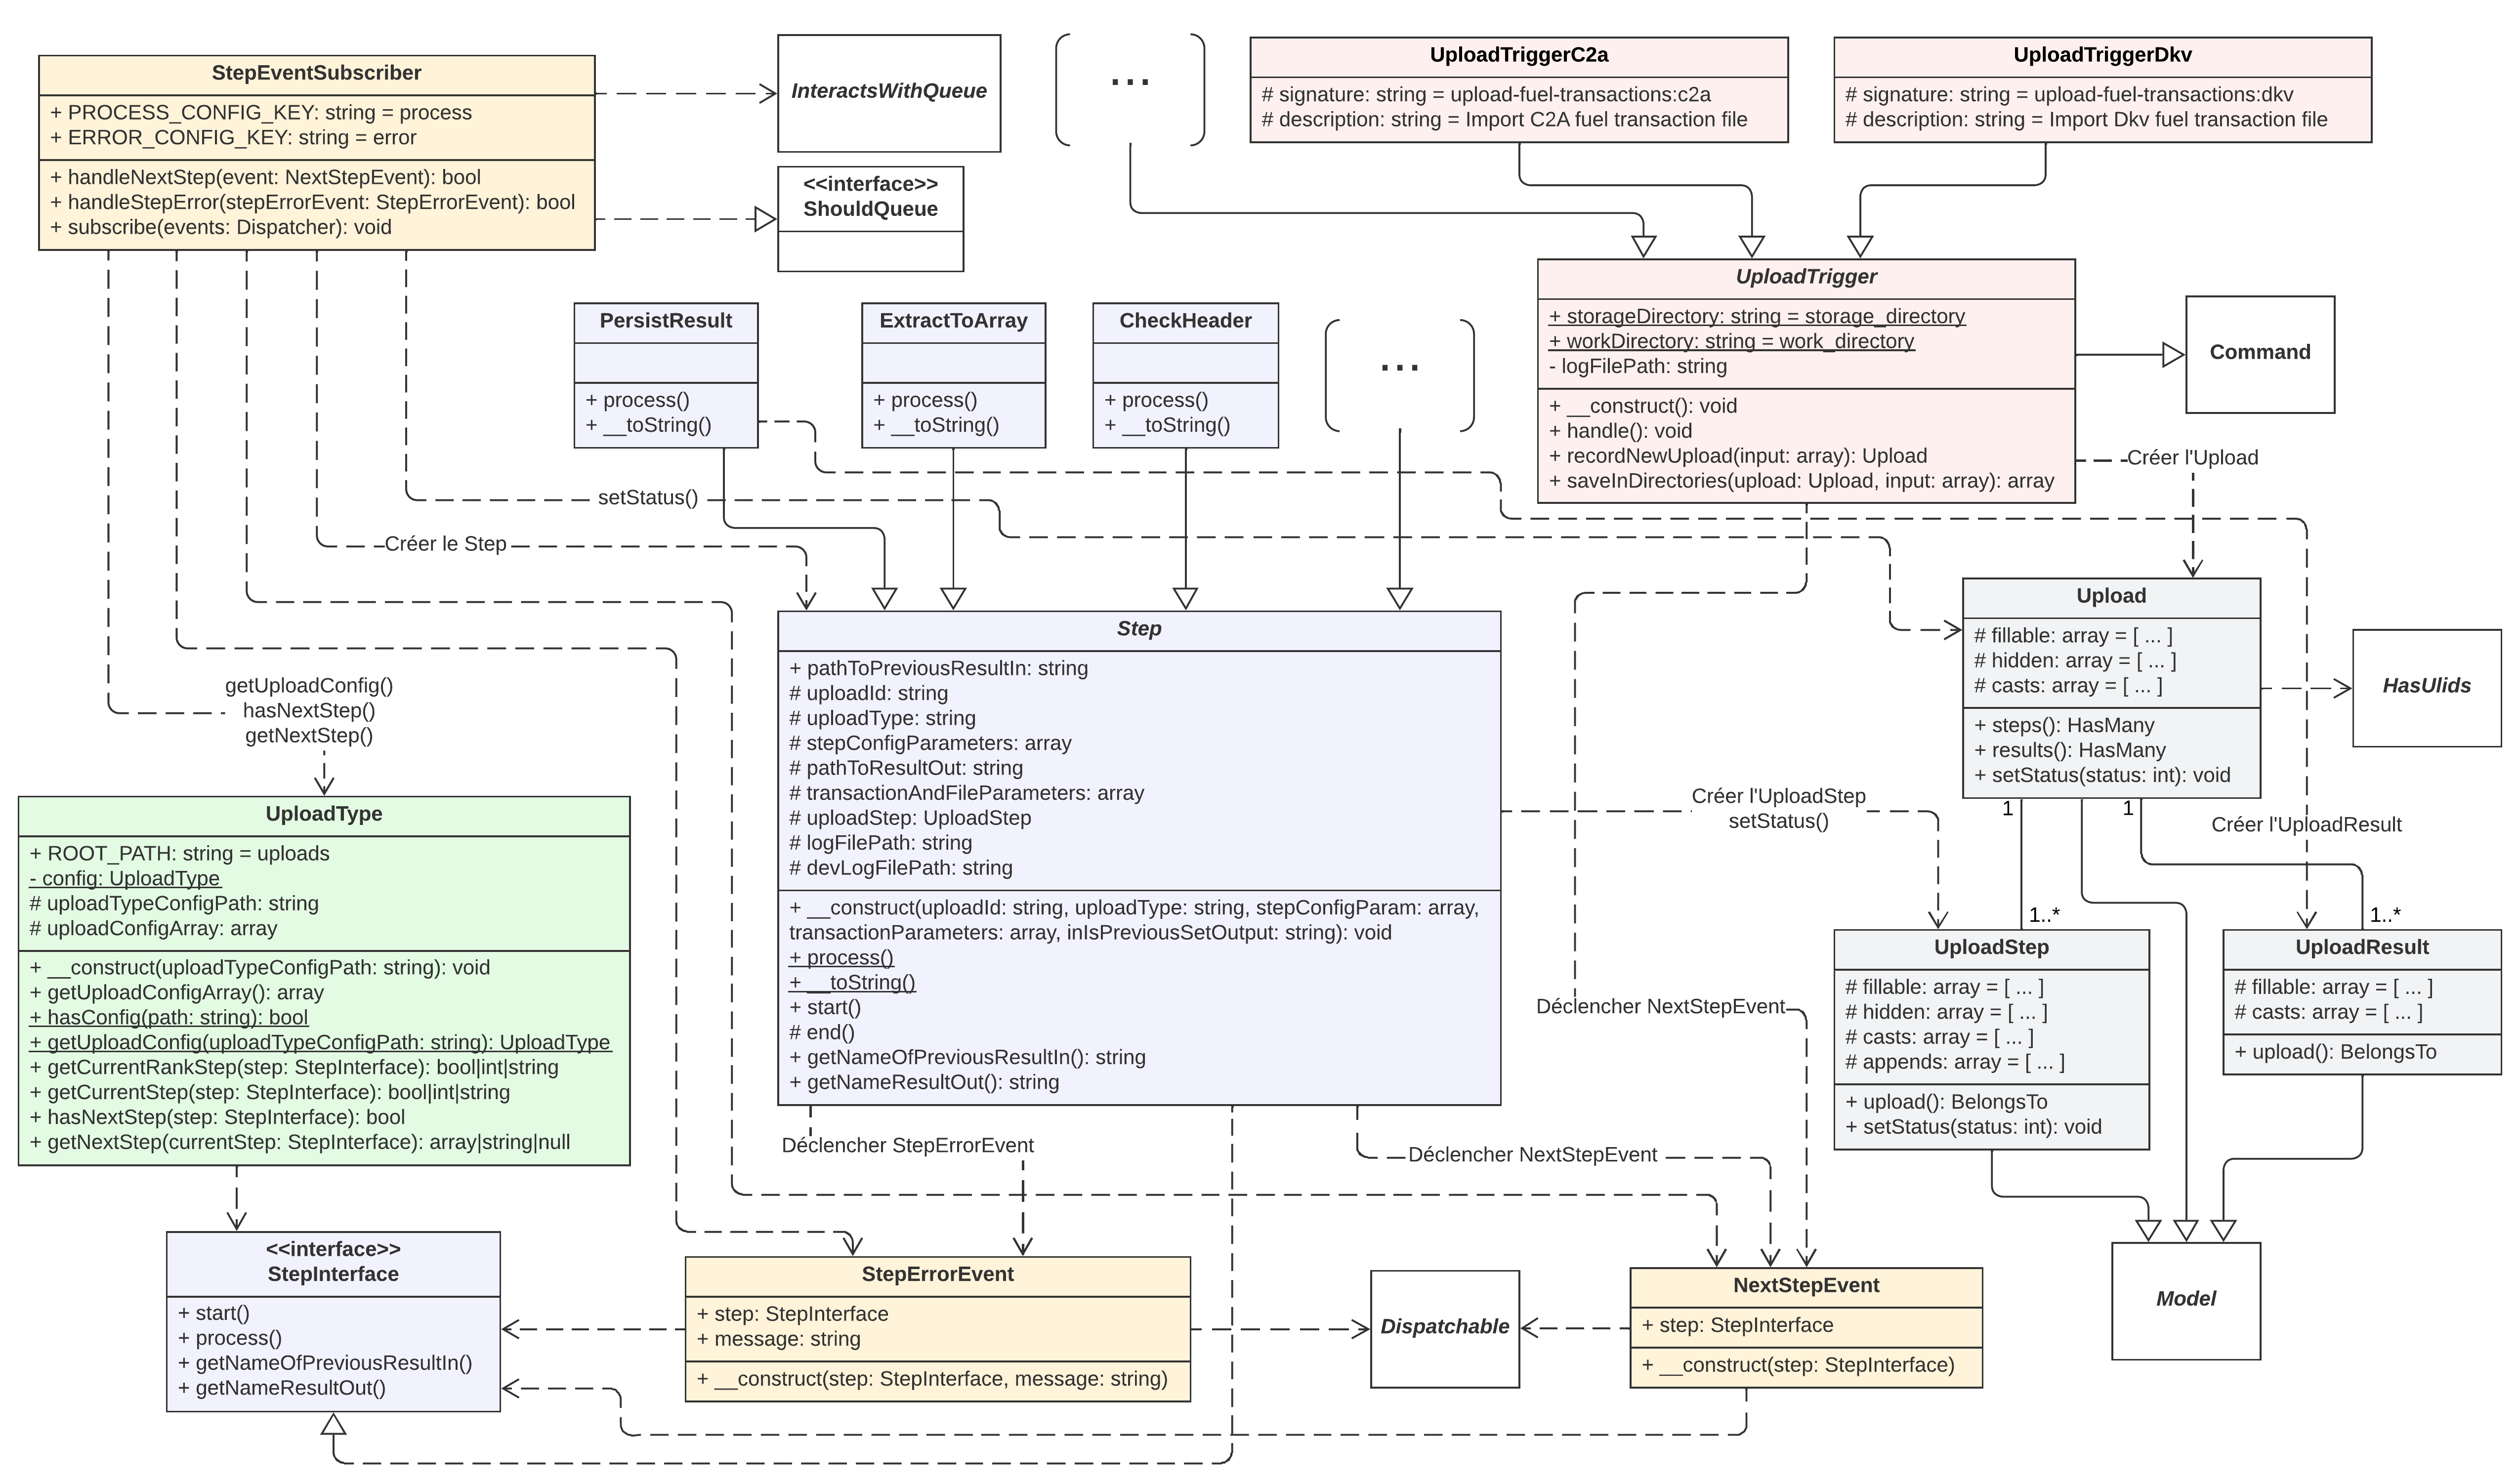
\includegraphics[width=\textwidth]{img/class-diagram-2}
    \caption{Diagramme des classes principales du Pipeline documentaire.}
    \label{fig:class-diagram}
\end{sidewaysfigure}

\begin{figure}
    \centering
    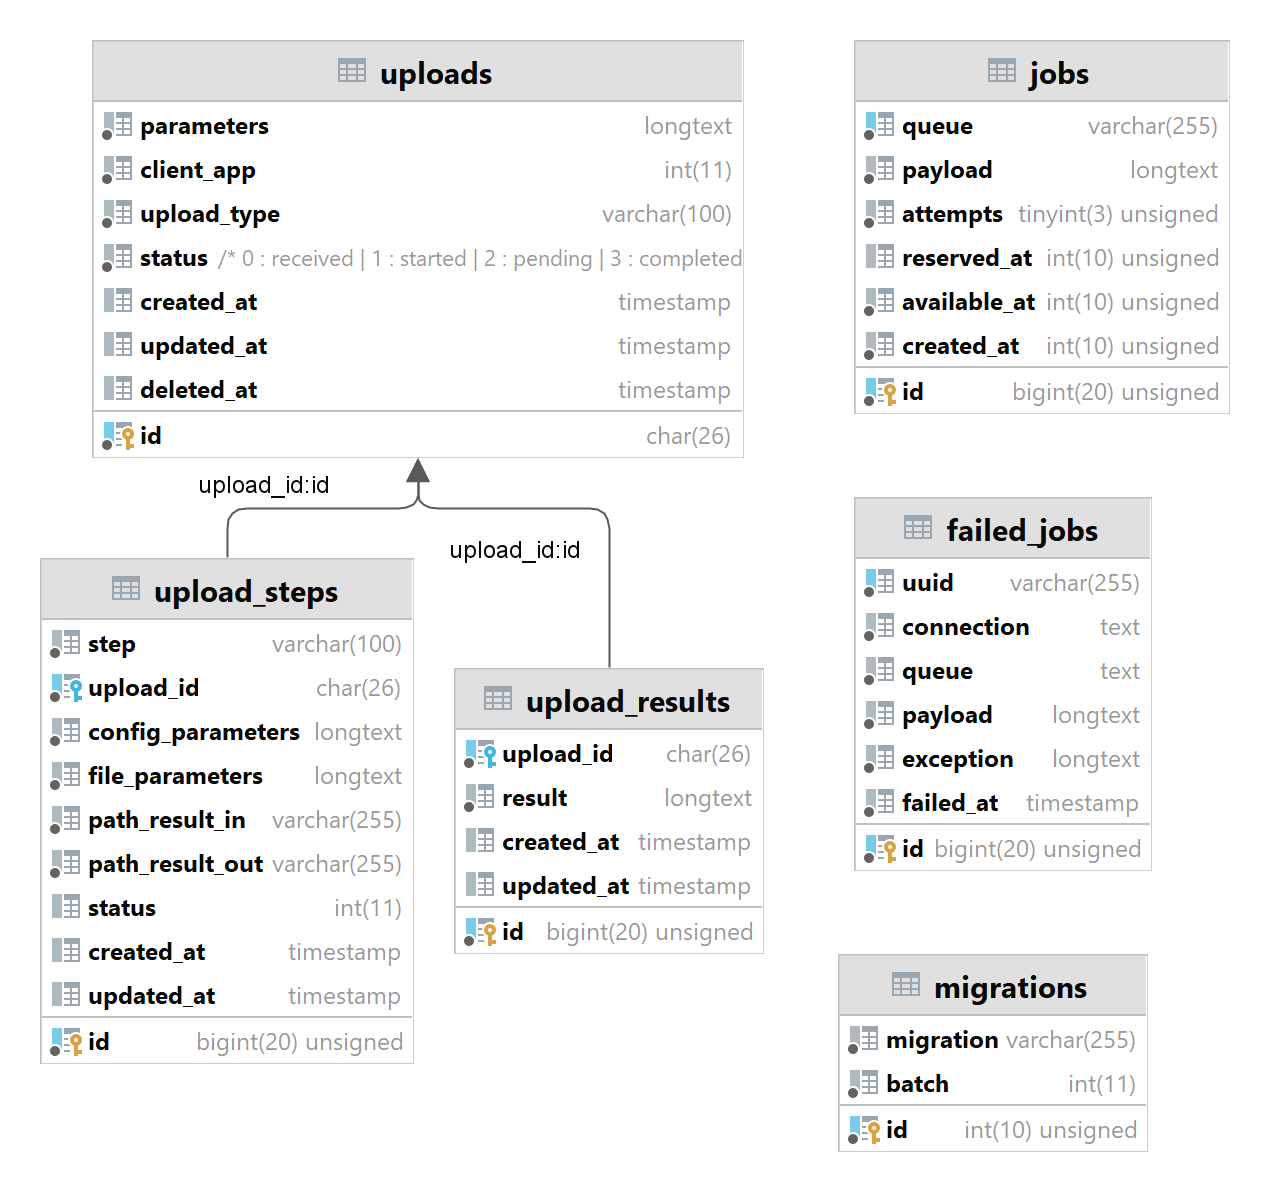
\includegraphics[width=\textwidth]{img/sdf_db}
    \caption{Modèle physique des données du Pipeline documentaire.}
    \label{fig:mpd}
\end{figure}